% 30-60-90 边比 1 : √3 : 2 （从等边切半推出）
\documentclass[tikz,border=4pt]{standalone}
\usepackage{ctex}
\usepackage{amsmath}
\begin{document}
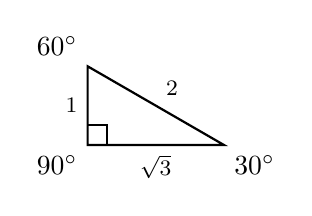
\begin{tikzpicture}[scale=1.0, thick]
  % 30-60-90: 短边 1（对 30°），长边 √3（对 60°），斜 2
  \coordinate (A) at (0,0);            % 90°
  \coordinate (B) at ({sqrt(3)}, 0);   % 60° at B? 实际上：角度对边。30° 对 1，60° 对 √3，90° 对 2.
  \coordinate (C) at (0, 1);
  % 重新：让 A=直角(原点)，对边斜边 BC=2；B 在 x 轴, C 在 y 轴
  % 取 AB=√3 (60° 在 C), AC=1 (30° 在 B)
  \renewcommand{\arraystretch}{1}
  \coordinate (A) at (0,0);
  \coordinate (B) at ({sqrt(3)}, 0);
  \coordinate (C) at (0, 1);
  \draw (A) -- (B) -- (C) -- cycle;
  \draw (0.25,0) -- (0.25,0.25) -- (0,0.25);
  \node[below] at ({sqrt(3)/2}, 0)    {\footnotesize $\sqrt{3}$};
  \node[left]  at (0, 0.5)            {\footnotesize $1$};
  \node[above right] at ({sqrt(3)/2}, 0.5) {\footnotesize $2$};
  \node[below left]  at (A) {$90^\circ$};
  \node[below right] at (B) {$30^\circ$};
  \node[above left]  at (C) {$60^\circ$};
\end{tikzpicture}
\end{document}
